% Gráfico: Tempo Máximo LNS - Nodes Left
\begin{figure}[htbp]
\centering
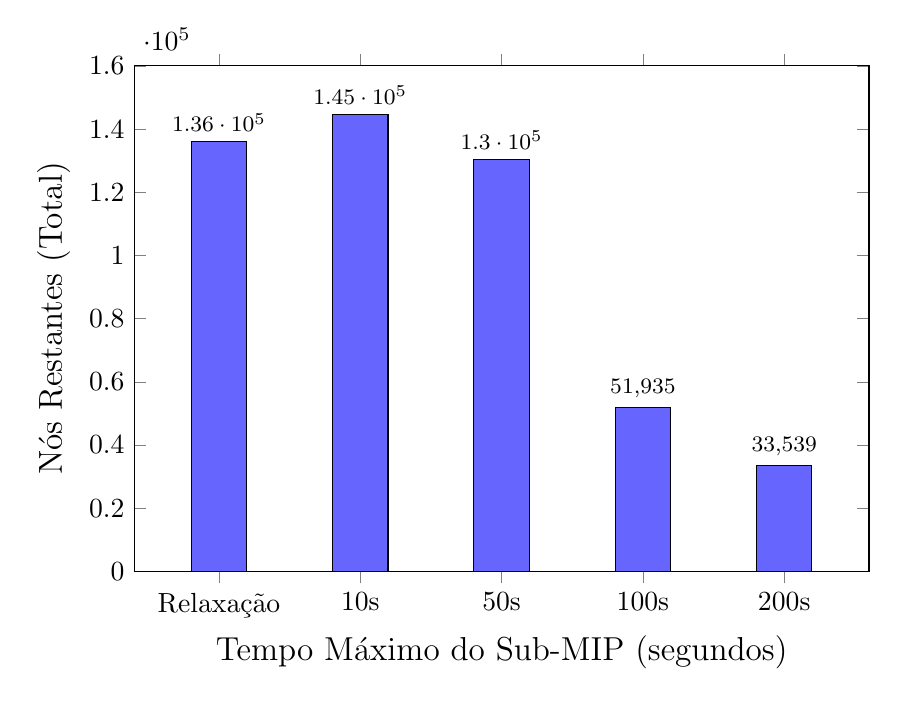
\begin{tikzpicture}
\begin{axis}[
    ybar,
    bar width=20pt,
    width=0.9\textwidth,
    height=8cm,
    ylabel={Nós Restantes (Total)},
    xlabel={Tempo Máximo do Sub-MIP (segundos)},
    symbolic x coords={Relaxação, 10s, 50s, 100s, 200s},
    xtick=data,
    nodes near coords,
    nodes near coords align={vertical},
    nodes near coords style={font=\footnotesize},
    ymin=0,
    ymax=160000,
    enlarge x limits=0.15,
    ylabel style={font=\large},
    xlabel style={font=\large},
    tick label style={font=\normalsize},
]
\addplot[fill=blue!60] coordinates {
    (Relaxação,135986)
    (10s,144674)
    (50s,130424)
    (100s,51935)
    (200s,33539)
};
\end{axis}
\end{tikzpicture}
\caption{Impacto do limite de tempo do sub-MIP no número de nós restantes. A configuração de 200s demonstrou o melhor desempenho com 33.539 nós, representando uma redução de 75,3\% em relação à relaxação pura.}
\label{fig:nodes_time}
\end{figure}
